\documentclass[12pt, letterpaper]{report} 
\usepackage[margin=0.5in]{geometry} %defined paper below
\usepackage[utf8]{inputenc}
\usepackage{blindtext}
\usepackage[usenames,dvipsnames]{xcolor} %adds mucho colors

%%%%%%%%%%%%%%%%%%%%%%%%%%%URLs%%%%%%%%%%%%%%%%%%%%%%%%%%%%%%%%%%%%
\usepackage{hyperref}
\hypersetup{
    colorlinks=true,
    linkcolor=blue,
    filecolor=magenta,      
    urlcolor=blue,
    pdfpagemode=FullScreen,
    }

\urlstyle{same} %%keeps the URL font same as text

%%%%%%%%%%%%%%%%%%%%%%%%%%%%%%%%%%%%%%%%%%%%%%%%%%%%%%%%%%%%%%%%%%%%
%%%%%%%%%%%%%%%%%%%%%%%%%%%Math Package%%%%%%%%%%%%%%%%%%%%%%%%%%%%%

\usepackage{amsmath}
\usepackage{amssymb}
\usepackage{amsthm}
\usepackage{graphicx}
\usepackage[mathscr]{eucal} %produce a script H, (for Hilbert Space or Laplace Transform)
\usepackage{tasks} %allows nice lists https://tex.stackexchange.com/a/324740

%%%%%%%%%%%%%%%%%%%%%%%%%%%%%%%%%%%%%%%%%%%%%%%%%%%%%%%%%%%%%%%%%%%%
%%%%%%%%%%%%%%%%%%%%%%%%%%%%%%%%%%%%%%%%%%%%%%%%%%%%%%%%%%%%%%%%%%%%

%%%%%%%%%included for CS%%%%%%%%%%%%%%%%%%%%%%

\usepackage{listings}
\usepackage{color}

\definecolor{dkgreen}{rgb}{0,0.6,0}
\definecolor{gray}{rgb}{0.5,0.5,0.5}
\definecolor{mauve}{rgb}{0.58,0,0.82}

\lstset{frame=tb,
  language={[latex]TeX}, %%change to your preferred language
  aboveskip=1mm,
  belowskip=1mm,
  showstringspaces=false,
  columns=flexible,
  basicstyle={\small\ttfamily},
  numbers=left,
  numberstyle=\tiny\color{gray},
  keywordstyle=\color{blue},
  commentstyle=\color{dkgreen},
  stringstyle=\color{mauve},
  breaklines=true,
  breakatwhitespace=true,
  tabsize=3
}

%%%%%%%%%%%%end of CS additions%%%%%%%%%%%%%%%



%%%%%%%%%%%%%%%%%%%%%%%%%%%%%%%%%%%%%%%%%%%%%%%%%%%%%%%%%%%%%%%%%%%%
%%%%%%%%%%%%%%%%%%%%%%%%%%%%%%%%%%%%%%%%%%%%%%%%%%%%%%%%%%%%%%%%%%%%

\usepackage{enumitem} %allows to resume enumeration
\usepackage{tabu} %allows tables using tabu
\usepackage{standalone}
\usepackage{tasks}

\usepackage{tikz}
\usetikzlibrary{decorations.pathreplacing}
\usepackage{tikz-network}
\usetikzlibrary{matrix}

\usetikzlibrary{arrows.meta,shapes,automata,backgrounds,petri,positioning}
\usetikzlibrary{decorations.pathmorphing}
\usetikzlibrary{decorations.shapes}
\usetikzlibrary{decorations.text}
\usetikzlibrary{decorations.fractals}
\usetikzlibrary{decorations.footprints}
\usetikzlibrary{calc}
\usetikzlibrary{spy}
\usetikzlibrary{arrows}
\usepackage{mathtools,etoolbox}

\usepackage{parskip} %something about paragraph lines
%defines columns
\usepackage{multicol}
\setlength{\columnsep}{1cm}


\usepackage{wrapfig} %able to insert pictures in text
\usepackage{gensymb} %allows the degree symbol for weather or angles
\usepackage{epigraph} %adds little quote start of chapter
\usepackage{systeme}%something about allowing system of equations stuff

\usepackage{pdfpages} %allows for import of separate files


\usepackage[framemethod=TikZ]{mdframed} %allows framed definitions

%%%%%%%%%%%%%%%%%%%%%%THEOREM BOXES%%%%%%%%%%%%%%%%%%%%%%%%%%%%%%
\newcounter{theo}\setcounter{theo}{0}
%\renewcommand{\thetheo}{\arabic{chapter}.\arabic{theo}}
\newenvironment{theo}[2][]{%
						\refstepcounter{theo}%
						\ifstrempty{#1}%
						{\mdfsetup{%
						frametitle={%
						\tikz[baseline=(current bounding box.east),outer sep=0pt]
						\node[anchor=east,rectangle,fill=JungleGreen!55]
						{\strut Theorem~\thetheo};}}
						}%
					{\mdfsetup{%
					frametitle={%
					\tikz[baseline=(current bounding box.east),outer sep=0pt]
					\node[anchor=east,rectangle,fill=JungleGreen!55]
					{\strut Theorem~\thetheo:~#1};}}%
						}%
					\mdfsetup{innertopmargin=10pt,linecolor=JungleGreen!55,%
					linewidth=2pt,topline=true,%
					frametitleaboveskip=\dimexpr-\ht\strutbox\relax
					}
\begin{mdframed}[]\relax%
\label{#2}}{\end{mdframed}}
%%%%%%%%%%%%%%%%%%%%%%%%%%%%%%%%%%%%%%%%%%%%%%%%%%%%%%%%%%%%%%%%

%%%%%%%%%%%%%%%%%%%%%%DEFINTION BOXES%%%%%%%%%%%%%%%%%%%%%%%%%%%
\newcounter{defi}[chapter] \setcounter{defi}{0}
\renewcommand{\thedefi}{\arabic{chapter}.\arabic{defi}}
\newenvironment{defi}[2][]{%
						\refstepcounter{defi}%
						\ifstrempty{#1}%
						{\mdfsetup{%
						frametitle={%
						\tikz[baseline=(current bounding box.east),outer sep=0pt]
						\node[anchor=east,rectangle,fill=WildStrawberry!55]
						{\strut Definition~\thedefi};}}
						}%
					{\mdfsetup{%
					frametitle={%
					\tikz[baseline=(current bounding box.east),outer sep=0pt]
					\node[anchor=east,rectangle,fill=WildStrawberry!55]
					{\strut Definition~\thedefi:~#1};}}%
						}%
					\mdfsetup{innertopmargin=10pt,linecolor=WildStrawberry!55,%
					linewidth=2pt,topline=true,%
					frametitleaboveskip=\dimexpr-\ht\strutbox\relax
					}
\begin{mdframed}[]\relax%
\label{#2}}{\end{mdframed}}
%%%%%%%%%%%%%%%%%%%%%%%%%%%%%%%%%%%%%%%%%%%%%%%%%%%%%%%%%%

%%%%%%%%%%%%%%%% Steps %%%%%%%%%%%%%%%%%%%%%%%%%%%%%%%%%%%

\newcounter{proc}[section] \setcounter{proc}{0}
\renewcommand{\theproc}{ }
\newenvironment{proc}[2][]{%
						\refstepcounter{proc}%
						\ifstrempty{#1}%
						{\mdfsetup{%
						frametitle={%
						\tikz[baseline=(current bounding box.east),outer sep=0pt]
						\node[anchor=east,rectangle, rounded corners,fill=RoyalBlue!60]
						{\strut PS~};}}
						}%
					{\mdfsetup{%
					frametitle={%
					\tikz[baseline=(current bounding box.east),outer sep=0pt]
					\node[anchor=east,rectangle, rounded corners,fill=RoyalBlue!60]
					{\strut PS~:~#1};}}%
						}%
					\mdfsetup{roundcorner=5pt, innertopmargin=10pt,linecolor=RoyalBlue!60, %
					linewidth=2pt,topline=true,%
					frametitleaboveskip=\dimexpr-\ht\strutbox\relax
					}
\begin{mdframed}[]\relax%
\label{#2}}{\end{mdframed}}
%%%%%%%%%%%%%%%%%%%%%%%%%%%%%%%%%%
%%%%%%%%%% Custom Section %%%%%%%%
\usepackage{titlesec}
  \titleformat{\section}
    {\normalfont\bfseries}{\thesection}{1em}{}[{\titlerule[.8pt]}]


%%%%%%%%%%%%%%%%%%%%%%%%%%%%% Tasks%%%%%%%%%%%%%%%%%%%%%%%%%%%%%%%%
\settasks{label-format={\color{green!70!black}\bfseries}, label-align=center, label-offset={5mm}, label-width={10mm}, item-indent={2mm}, item-format={\scshape\small}, column-sep={3mm}, after-item-skip=1mm, after-skip={3mm}
}
%%%%%%%%%%%%%%%%%%%%%%%%%%%%%%%%%%%%%%%%%%%%%%%%%%%%%%%%%%%%%%%%%%%


\newcommand{\ds}{\displaystyle}
\newcommand{\ra}{\rightarrow}
\newcommand{\Ra}{\Rightarrow}
\newcommand{\Lra}{\Leftrightarrow}
\newcommand{\mc}{\mathcal}
\newcommand{\mrm}{\mathrm}
\newcommand{\ul}{\underline}
\newcommand{\ol}{\overline}
\newcommand{\cl}{\overline}
\newcommand{\hs}{\hspace}
\newcommand{\vs}{\vspace}

%%%%%%%%%%%%%%%%%%%Topology%%%%%%%%%%%%%%%%%%%%%%%%%%%%
\newcommand{\interior}[1]{\mathrm{int(#1)}}
\newcommand{\bdy}[1]{\mathrm{bdy(#1)}}
\newcommand{\inter}[1]{#1^{\mathsf{o}}}
%\newcommand{\closure}[1]{\ol{#1}} % simple
\newcommand{\closure}[2][3]{{}\mkern#1mu\ol{\mkern-#1mu#2}} %nicer on eyes
\DeclarePairedDelimiterX{\abs}[1]{\lvert}{\rvert}{\ifblank{#1}{{}\cdot{}}{#1}} %absolute value bars

\def\T{\mathcal{T}}
\def\K{\mathcal{K}}
\def\s{\mathcal{S}}
\def\U{\mathscr{U}}
\def\V{\mathscr{V}}
\def\B{\mathcal{B}}

\newcommand{\metspace}[2]{({#1},{#2})-\mbox{metric space}}
\newcommand{\ms}[2]{({#1},{#2})}
\newcommand{\ts}[2]{({#1},{#2})}

\newcommand{\genfunc}[3]{{#3}\colon {#1} \longrightarrow {#2}}
\newcommand{\genfuncdef}[5]{{#3} \colon {#1} \longrightarrow {#2}\mbox{ where } {#4} \mapsto {#5} }


%%%%%%%%%%%%%%%%%% General %%%%%%%%%%%%%%%%%%%%%%%%%%%%


\newcommand{\rsphere}{\mathbb{C}_\infty}
\newcommand{\Disk}{\mathbb{D}}
\newcommand{\disk}{\Delta}
\newcommand{\wh}{\widehat}
\newcommand{\e}{\varepsilon}
\newcommand{\0}{\emptyset}

\newcommand{\bd}{\partial}
\newcommand{\im}{\mathrm{Im}}
\newcommand{\pr}{\mathrm{Pr}}
\newcommand{\sh}{\mathrm{Sh}}
\newcommand{\dm}{\mathrm{diam}}
\newcommand{\dist}{\mathrm{d}}
\newcommand{\sm}{\setminus}

\newcommand{\tp}[1]{\textcolor{violet}{\textbf{\emph{#1}}}}
\newcommand{\tb}[1]{\textcolor{TealBlue!80!black}{\textbf{\emph{#1}}}}


\def\C{\mathbb{C}}
\def\R{\mathbb{R}}
\def\Q{\mathbb{Q}}
\def\N{\mathbb{N}}
\def\Z{\mathbb{Z}}




%defined theorems and definitions section
\theoremstyle{theorem}
\newtheorem{defn}{\emph{Definition}}

\theoremstyle{definition}
\newtheorem{ndefn}{Naive Definition}

\theoremstyle{definition}
\newtheorem{ex}{Example}

\theoremstyle{definition}
\newtheorem{DIY}{DIY}

\theoremstyle{definition}
\newtheorem{post}{Postulate}

\theoremstyle{theorem}
\newtheorem{thm}{Theorema}

\theoremstyle{theorem}
\newtheorem{cor}{Corollary}

\theoremstyle{remark}
\newtheorem{rmk}{Remark}

\begin{document}
\chapter{}

\section{Document Types}

There are numerous document types that exist to serve different purposes but in general we will use:

	\begin{itemize}
		\item \textbf{\emph{Report}}
		\item Exam
		\item Beamer
	\end{itemize}
	
	\begin{lstlisting}
			\documentclass[12pt, letterpaper]{report}
	\end{lstlisting}
	
	To learn more about different document types and their differences:  \href{http://www.overleaf.com}{Something Linky} \\ \\ 
	Or to learn about different parameters: 
	
	\url{https://texblog.org/2013/02/13/latex-documentclass-options-illustrated/}
	
\LaTeX \; is known as a \href{https://en.wikipedia.org/wiki/Markup_language#Descriptive_markup}{\emph{descriptive markup}} language, so a lot the commands you might need are called/labeled what you would usually expect.  At this point we have used things like:

	\begin{lstlisting}
		\chapter{First Document} %makes a chapter with the given title
		\section{Document Types} %similarly for section; 
		
			\begin{itemize} %creates an unordered list;
				\item				%we can customize these per \item 
			\end{itemize}

		\textbf{} 		%bold command
		\emph{}	  		%italics command
		\underline{}   %underline command
		
			\begin{lstlistings}
				 %this is imported using the \usepackage{listings}it allows us to write source code and customize, see this file source code as to how it was implemented here	
			\end{lstlistings}
			
		\href{} #vs. \url{} % \href allows for 'Clicky Label' meanwhile \url is the raw URL

		
		
	\end{lstlisting}
	
\section{Math Mode}

For many people the most useful part of LaTeX is the ability to typeset complex mathematical formulas.  Many commands and their applications with working examples can be found here: \href{http://tug.ctan.org/info/short-math-guide/short-math-guide.pdf}{Short Math Guide for \LaTeX}

Certain things require certain packages, for example, we need gensymb package in order to write the degree symbol appropriately: $5\degree$

	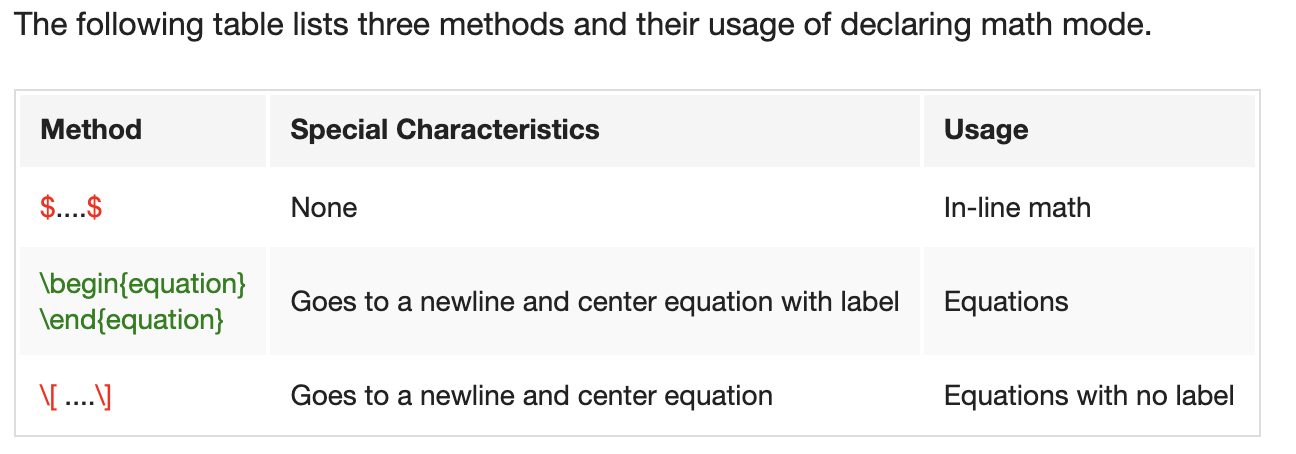
\includegraphics[width=\textwidth]{images/mathopt.png} %includes image found in the images folder

The most common packages are listed below and working examples are on the last page titled $$\mbox{``Definitions from Topology Lectures"} $$

	\begin{lstlisting}
		\usepackage{amsmath}
		\usepackage{amssymb}
		\usepackage{amsthm}
		\usepackage{graphicx}
		\usepackage[mathscr]{eucal} %produce a script H, (for Hilbert Space or Laplace Transform)
		
		\usepackage{mathtools,etoolbox}

		\usepackage{parskip} %something about paragraph lines
		
		%defines columns
		\usepackage{multicol}
		\setlength{\columnsep}{1cm}


		\usepackage{wrapfig} %able to insert pictures in text
		\usepackage{gensymb} %allows the degree symbol for weather or angles
		\usepackage{epigraph} %adds little quote start of chapter
		\usepackage{systeme}%something about allowing system of equations stuff
		
		$5\degree$ %displays math text within body of the text
		$$5\degree$$ %opens up math mode; similar to using \[ ... \]
	\end{lstlisting}

%notice here that two ticks ` instead of ' play with it so you keep it mind when it looks funny

	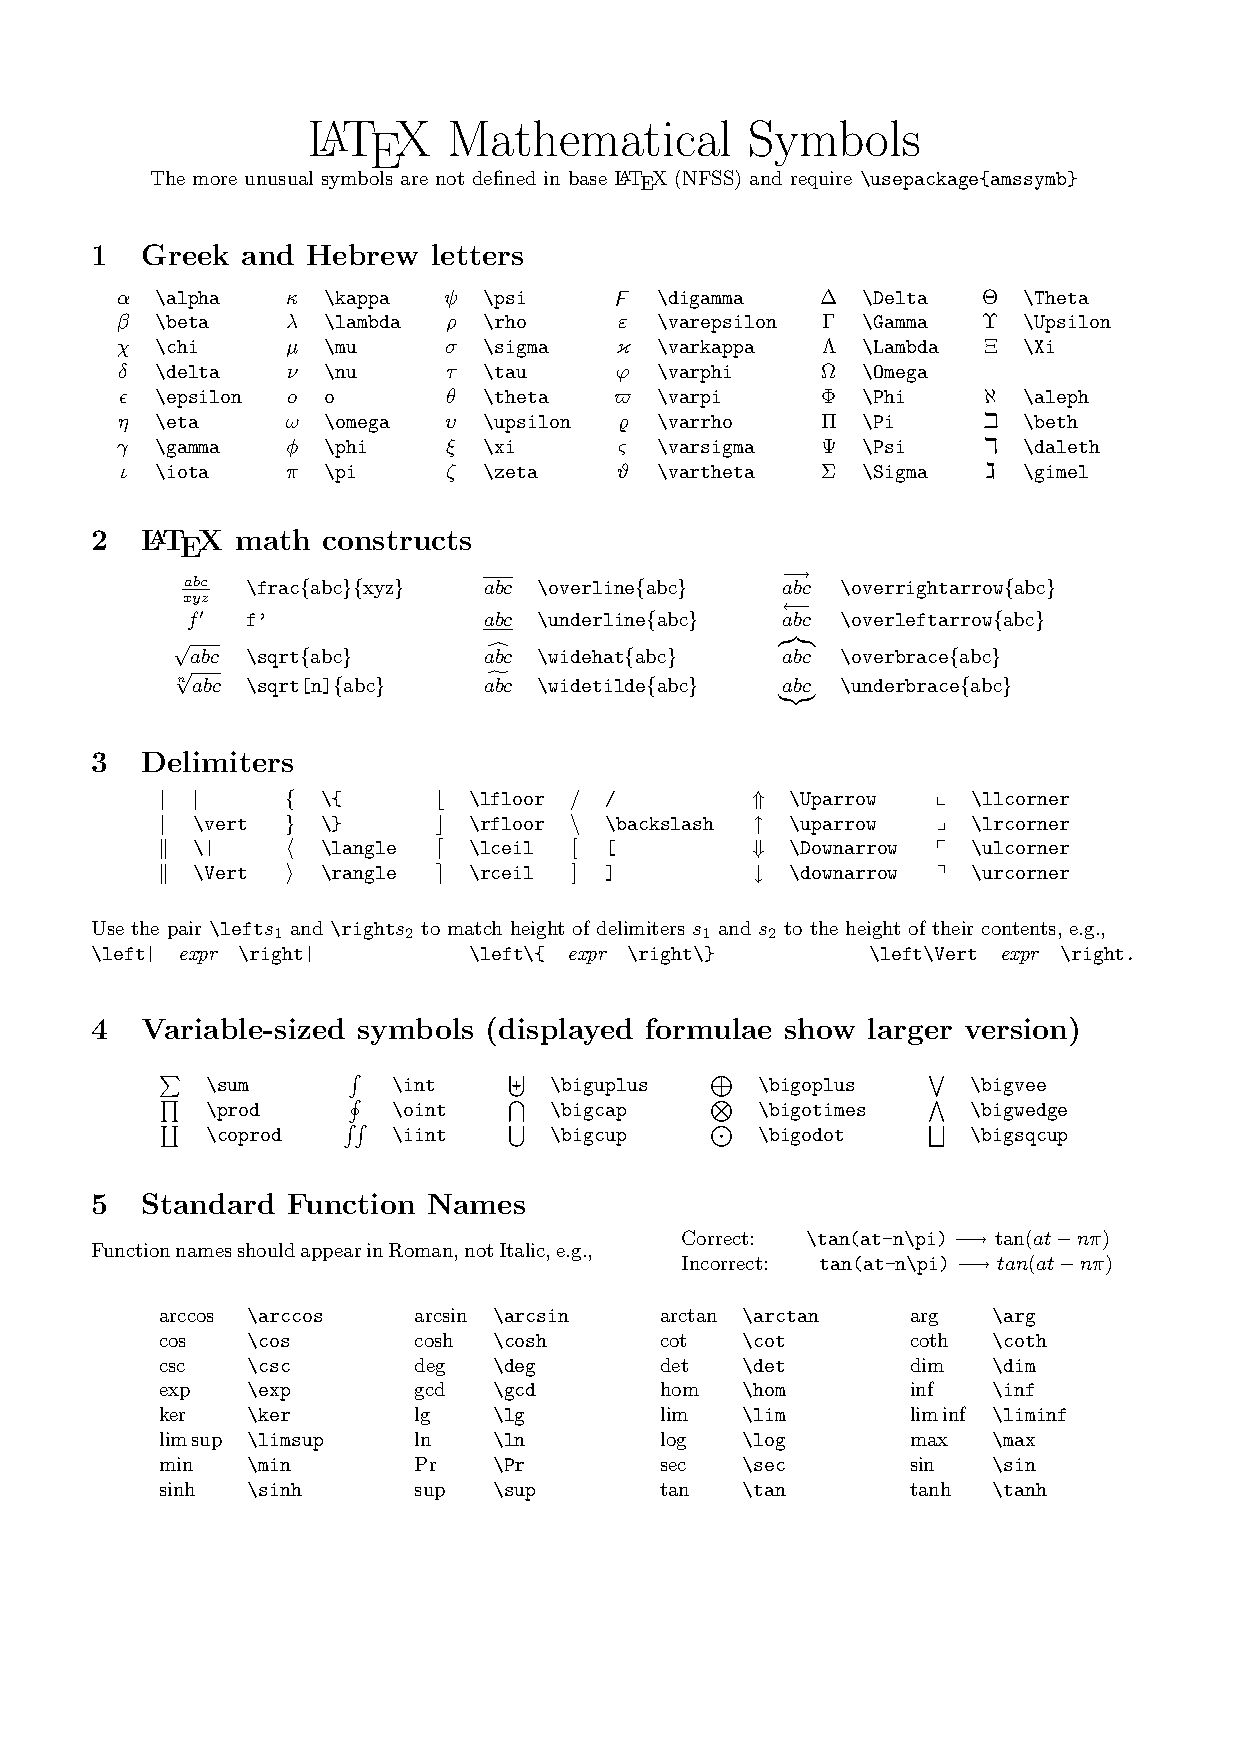
\includepdf[pages=-]{symbols.pdf} %imports entire pdf

\newpage

\textbf{Tikz package}

Another good example or a useful package is the tikz package whichs allows you to create your own graphs and charts.  This is far beyond my scope, but these are a few things I have created, so I feel its worth mentioning.

	\begin{lstlisting}
\usepackage{tikz}
	\usetikzlibrary{decorations.pathreplacing}
\usepackage{tikz-network}
	\usetikzlibrary{matrix}

	\usetikzlibrary{arrows.meta,shapes,automata,backgrounds,petri,positioning}
	\usetikzlibrary{decorations.pathmorphing}
	\usetikzlibrary{decorations.shapes}
	\usetikzlibrary{decorations.text}
	\usetikzlibrary{decorations.fractals}
	\usetikzlibrary{decorations.footprints}
	\usetikzlibrary{calc}
	\usetikzlibrary{spy}
	\usetikzlibrary{arrows}

	\end{lstlisting}
	
	\includestandalone[width=5in]{tikz-code/secline} %%include Tikz Graphic
	
	
	\newpage


\section{Importing Images and PDF's}
There will be time when you will need to import an image or a PDF, or perhaps only part of a PDF.

	\begin{lstlisting}
		\includestandalone[width=5in]{tikz-code/secline} %%include Tikz Graphic
		
		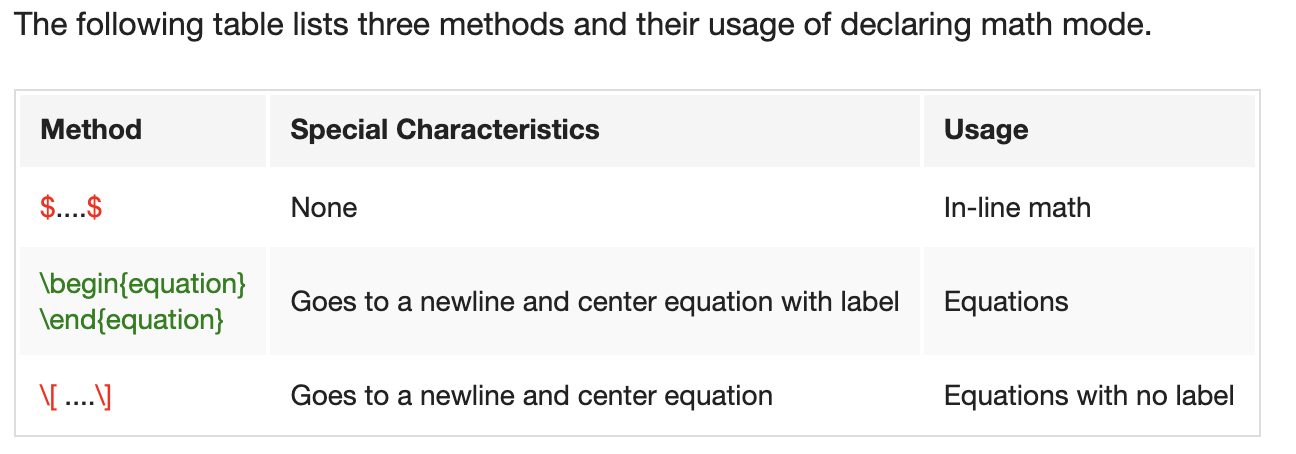
\includegraphics[width=\textwidth]{images/mathopt.png} 
		%includes image found in the images folder; this is what I use 90% as I use screenshots all the time.  
		
		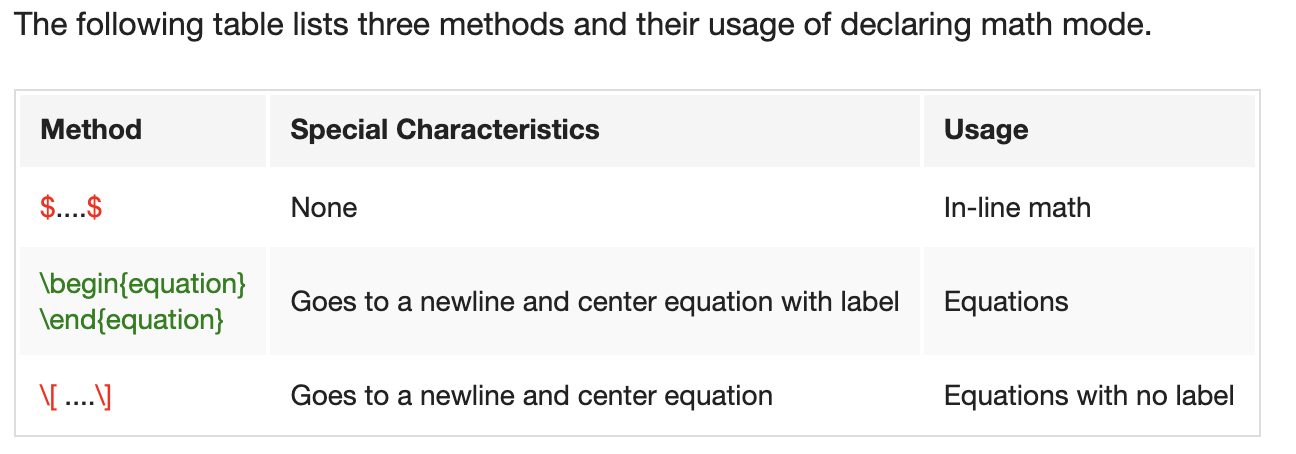
\includegraphics[width=0.5\textwidth]{images/mathopt.png} 
		%In general I use width=\textwidth and then multiply by some small value so that if fits to my needs
		
		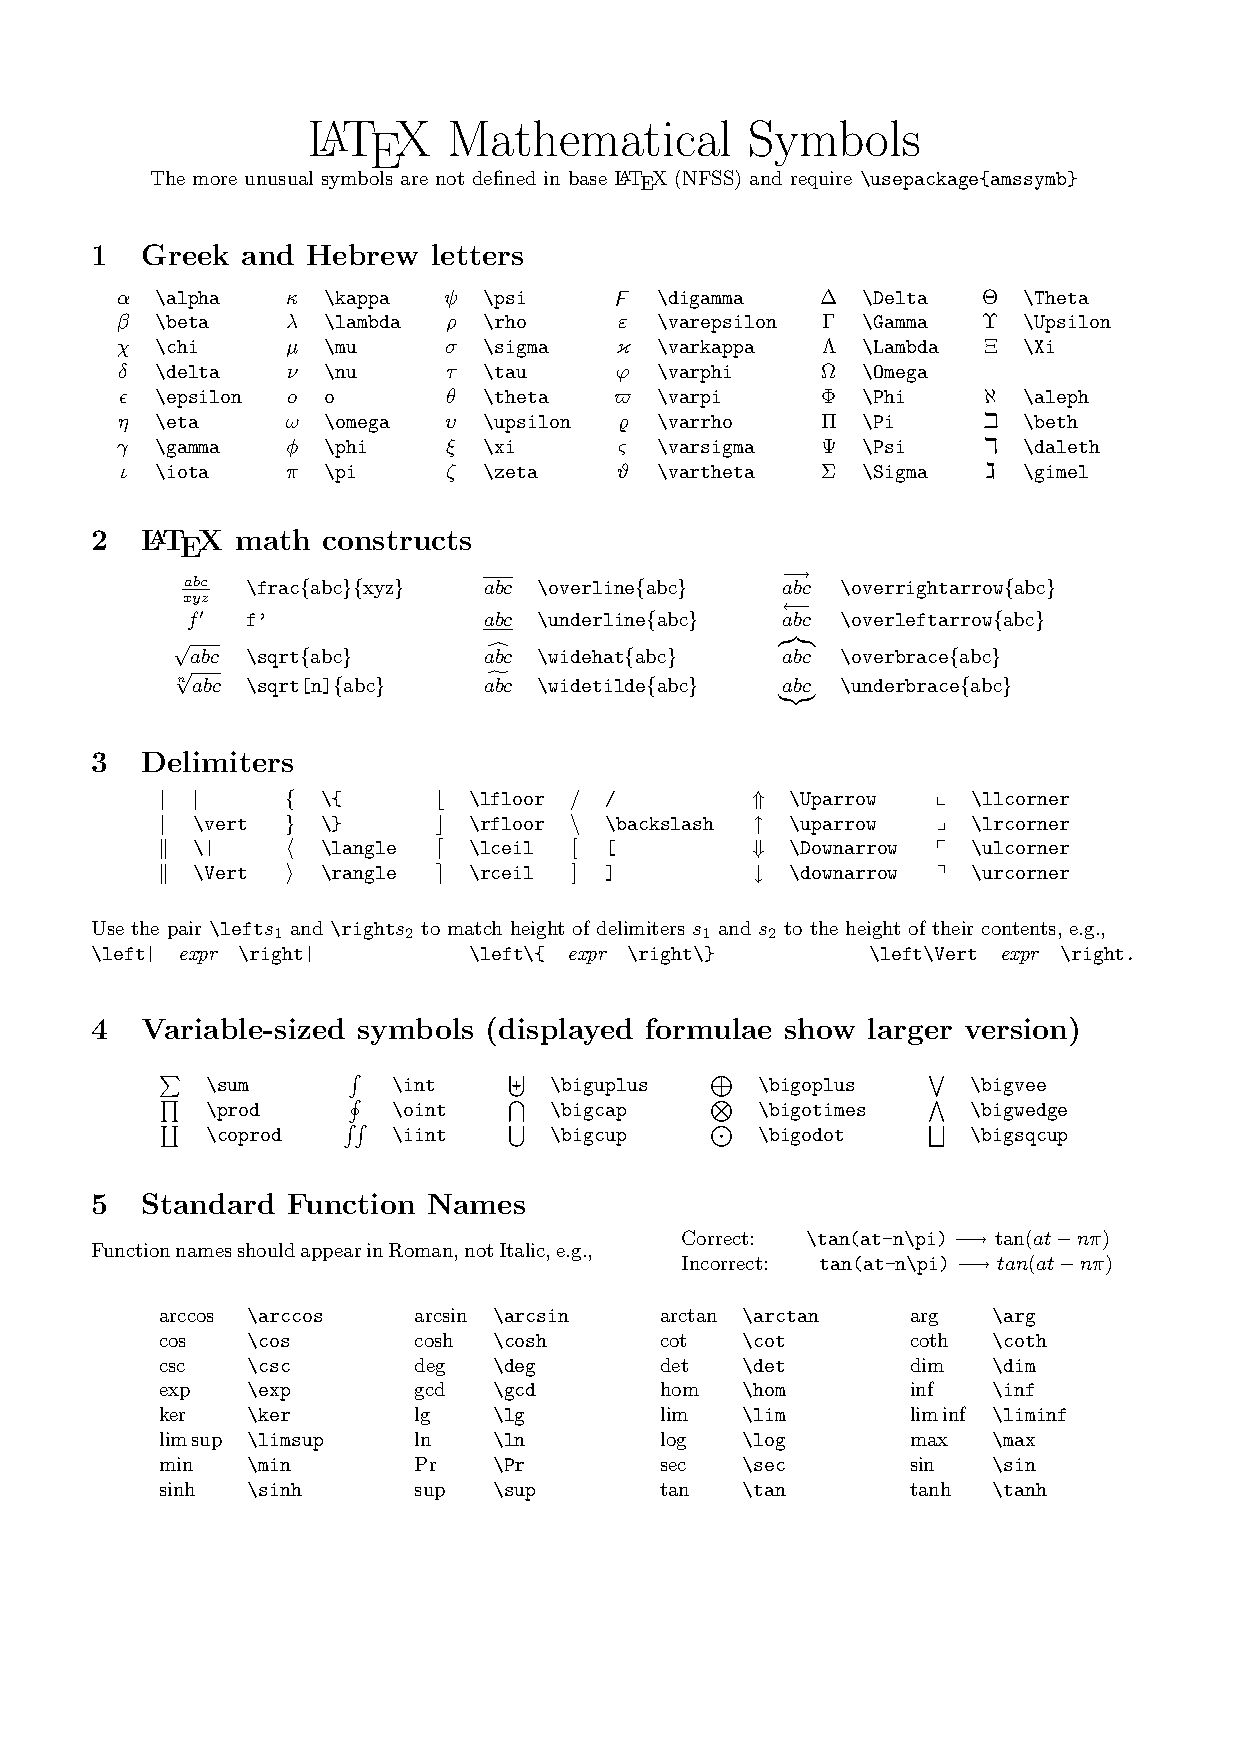
\includepdf{symbols.pdf} 		%imports only first page
		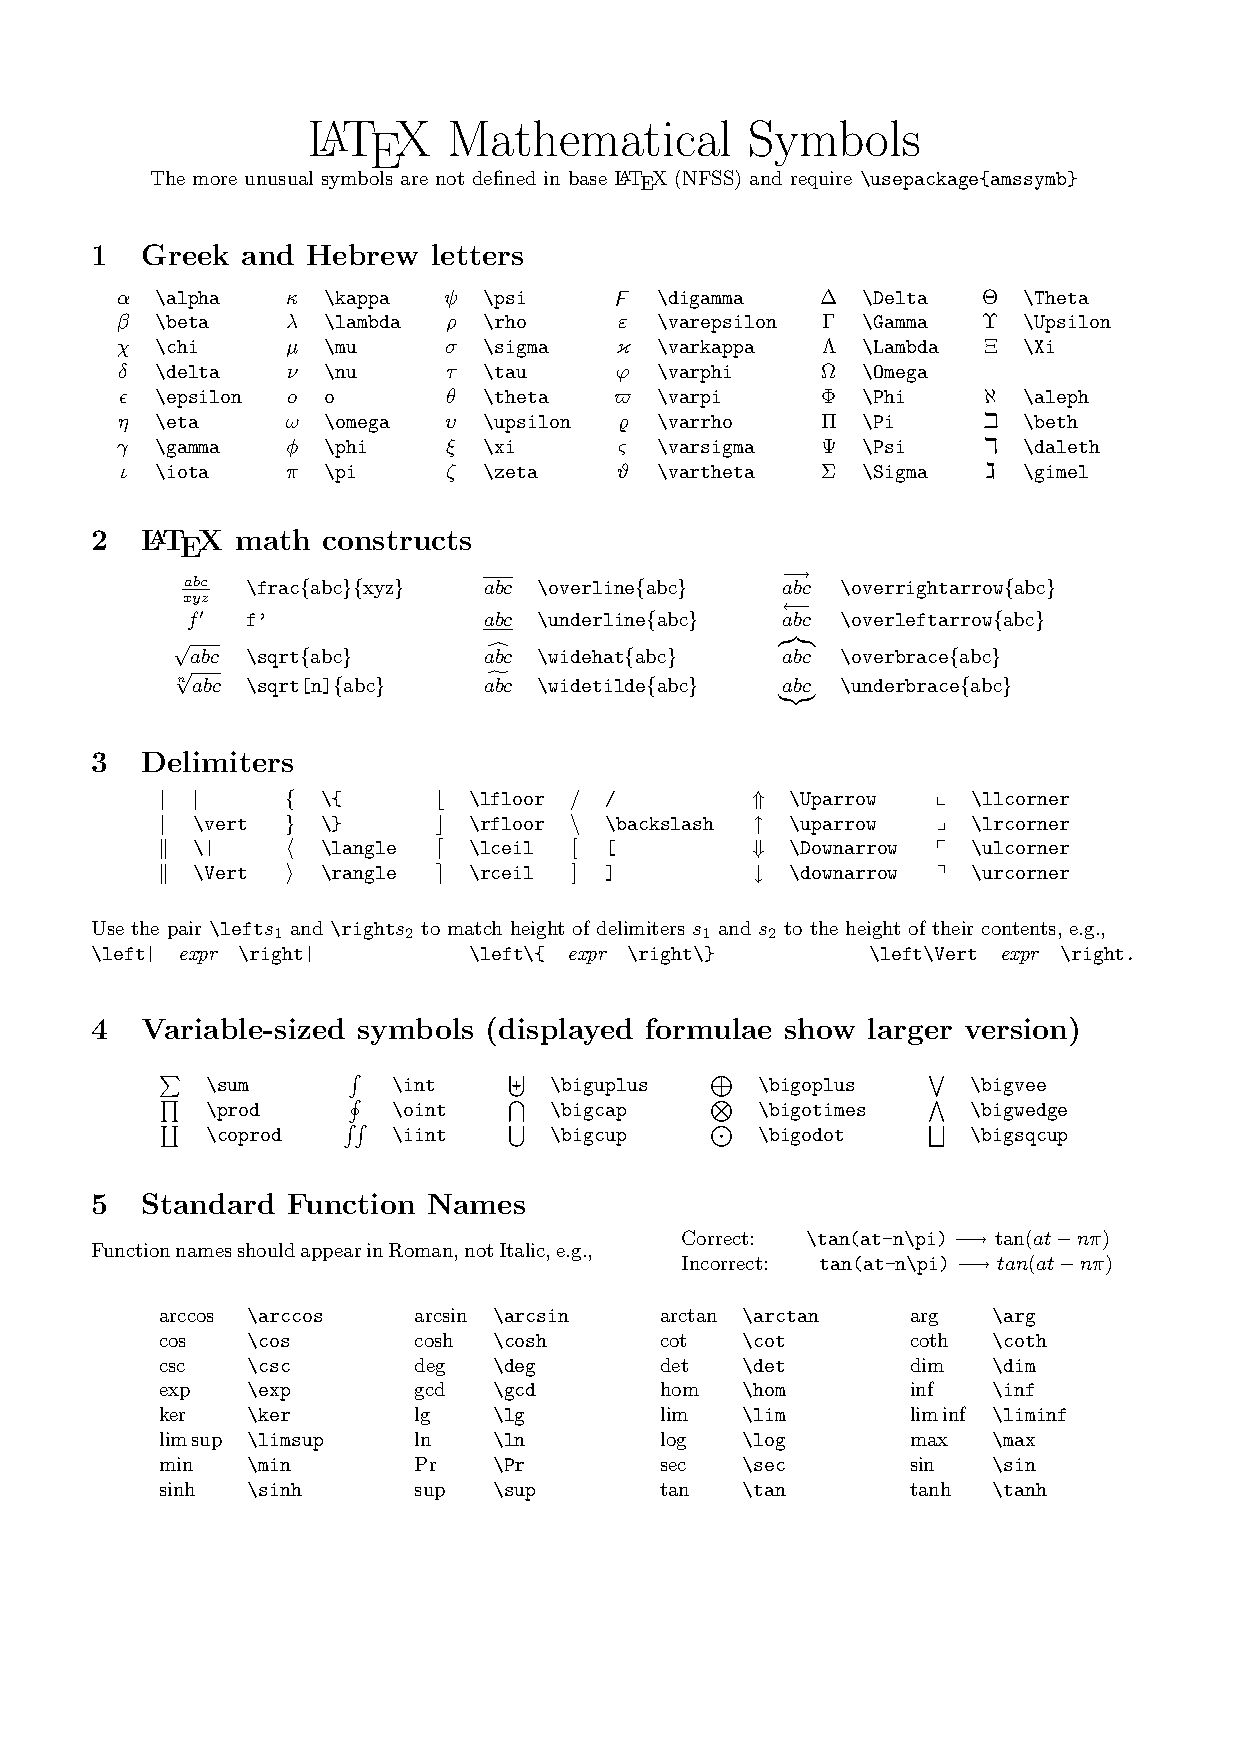
\includepdf[pages={1,3,5}]{symbols.pdf} %imports only pages 1,3,5
		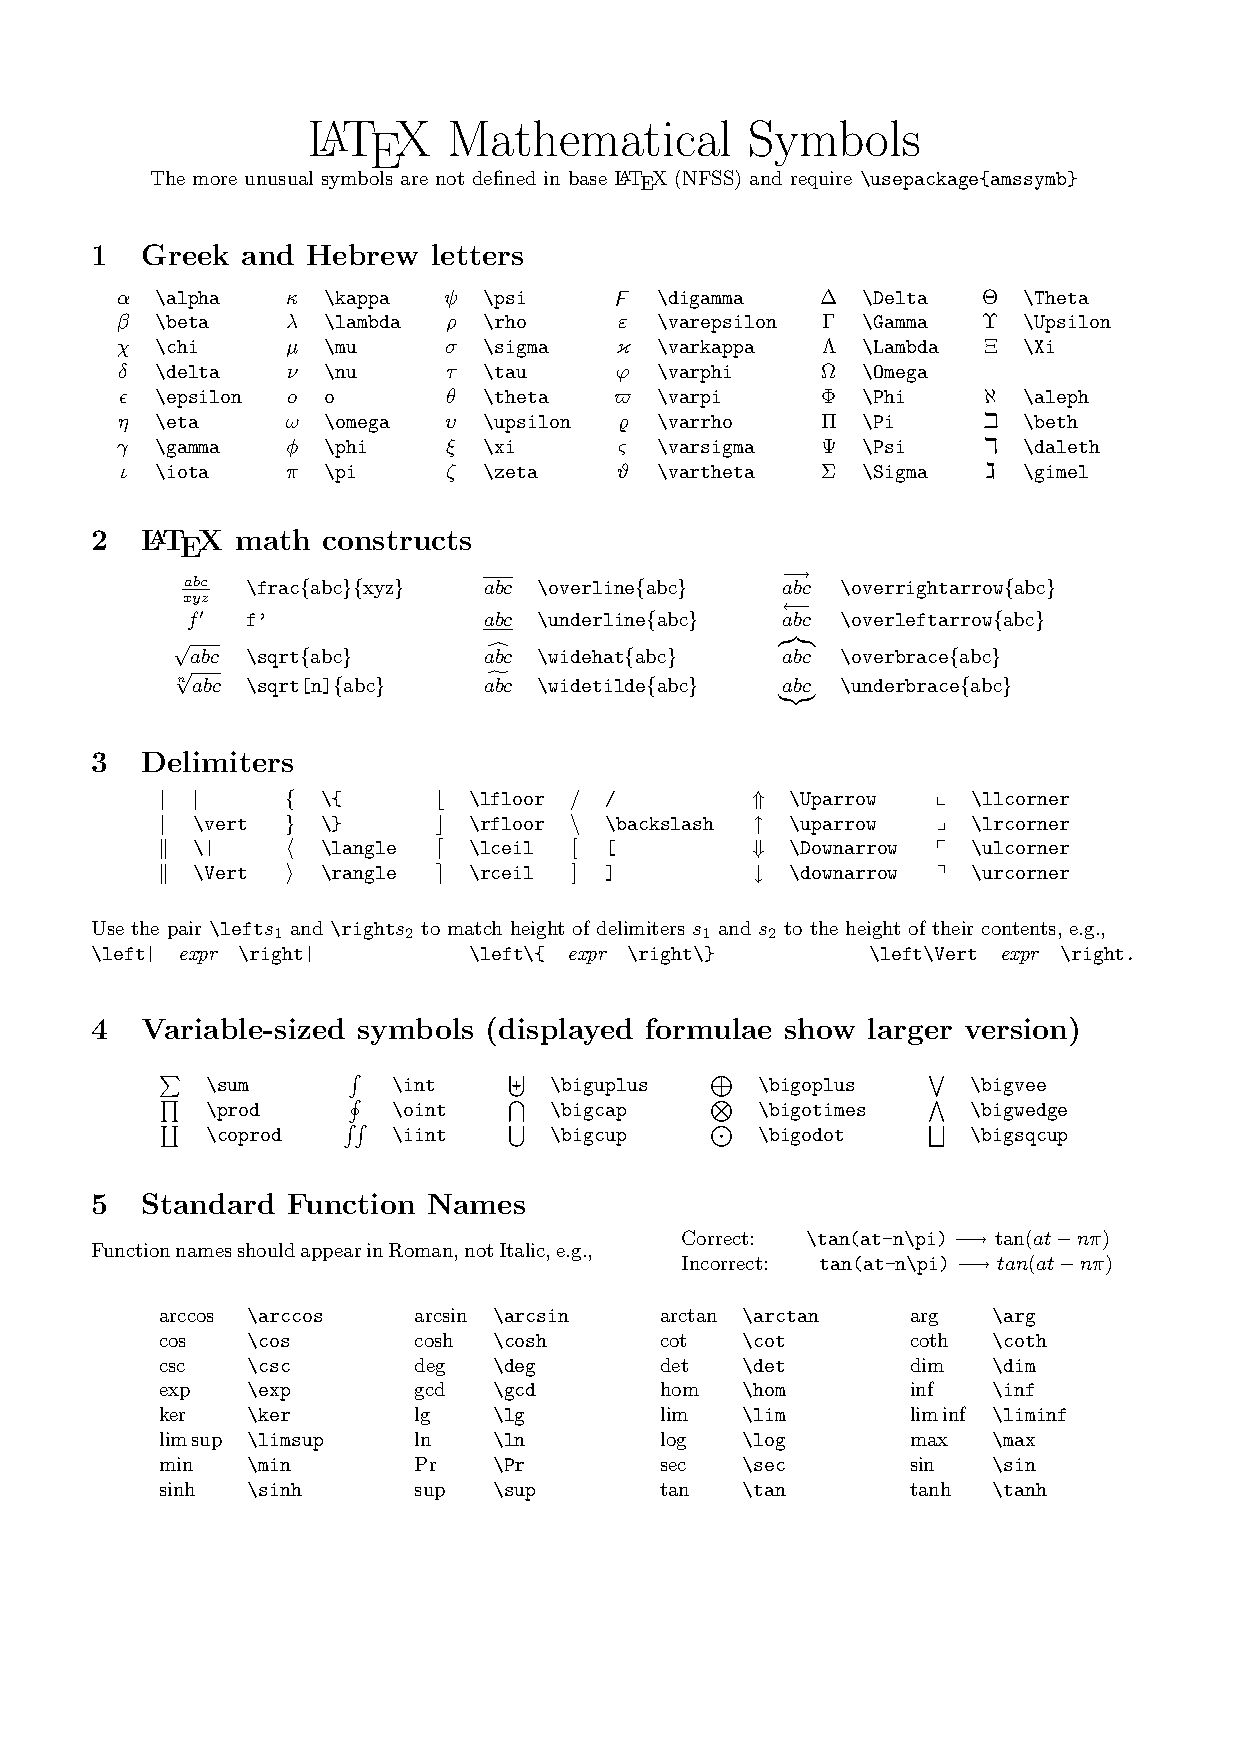
\includepdf[pages=-]{symbols.pdf} %imports entire pdf	
	\end{lstlisting}
	
	There are different parameters you can use in regards to width and height so I suggest you do some playing around with it and if you need something specific it probably already exists, you just need to use Google or just check out the \href{https://www.overleaf.com/learn/latex/Inserting_Images}{Inserting Images} resource on \url{https://www.overleaf.com/} website where you will find a lot of useful information.
	
	Luckily for us, the \LaTeX \; community found it convenient to also use similar labels for importing PDF's as well as Tikz that you want to directly import and update (just in case you decide to make big changes and forget to update the screenshot).
	
\section{Report versus Exam}

The report document type is what I use 9 out of 10 times; the exam document type is for that 1 out of 10.

I have used the report document class for the majority of my work due to its flexibility.  This file is a good example of the pre-amble I have built up and found the most useful over my 5 years of teaching.  There might be redundancies, or more efficient methods, but this is what I have created to fit my needs.  In general I have written a short comment to help me remember why I imported it in the first place as you don't always use certain packages.\footnote{A person could argue that this makes my file inefficient and larger than they need to be but eh, you can always delete a file of two... right?! \color{red}{(Also, this is how you include footnotes as well as color in your text.)}}

The key differences/benefits to using the exam document class when writing exams is that it has built in keywords such
	\begin{enumerate}
		\item \begin{verbatim}\question and \parts \end{verbatim}
		\item \begin{verbatim}\points \end{verbatim}
		\item \begin{verbatim} \gradetable, \bonusgradetable, \combinedgradetable \end{verbatim}
		\item Environments for Multiple Choice and Customization
	\end{enumerate}

If you understand how to use the itemize/enumerate to create (un)ordered lists, then the exam class will be a breeze to use.  This is the pre-amble I use for exams, as you will note, its way shorter than the one I use for reports. For more, go to \href{https://www.overleaf.com/learn/latex/Typesetting_exams_in_LaTeX}{Basics in Overleaf}.  I have included a few sample files in this repo so you can have a few sample exams/templates of what I used and how (I manipulated it to my needs).

	\begin{lstlisting}
	\documentclass[addpoints,12pt]{exam} %allows points and gradetable
	\usepackage{wrapfig} 
	\usepackage{graphicx}
	\usepackage{multicol}
	\usepackage{amsmath}
	\usepackage{wrapfig} %able to insert pictures in text
	\usepackage{gensymb} %allows the degree symbol for weather or angles
	\usepackage{enumitem}
	\usepackage{bigints} %large integral symbols LARGE INTEGRAL SYMBOLS!!!
	\usepackage[table,xcdraw]{xcolor}
	\usepackage{mathtools,etoolbox}
	\DeclarePairedDelimiterX{\abs}[1]{\lvert}{\rvert}{\ifblank{#1}{{}\cdot{}}{#1}}
	\newcommand\norm[1]{\left\lVert#1\right\rVert}
	
	\begin{document}
%%%%%% Cover Page for Exam%%%%%%%%
	\begin{center}
	\fbox{\fbox{\parbox{5.5in}{\centering
	EXAM NUMBER 2}}}
	
	\end{center}
	\noindent I acknowledge that I have read and agree to the Crespi Carmelite High School Academic Integrity Contract (page 24 of the Parent/Student Handbook), and I agree to complete this exam in accordance with the contract's stipulations. 
	
	\vspace{0.5in}
	\makebox[\textwidth]{Name and period:\enspace\hrulefill}
	
	\vspace{.5 in}
	\makebox[\textwidth]{Signature: \enspace\hrulefill}
	
	\vspace{1cm}
	
	\noindent \textbf{DO NOT BEGIN UNTIL INSTRUCTED TO DO SO}
	\noindent You have until the end of the period to finish this exam.  If you happen to finish early please have a seat until the end of the period. The exam is worth \textbf{100 points}. You are allowed to write on this exam.
	
	\newpage
%%%%%%% First Page of Exam %%%%%%%%%%%%	
	\begin{center}
	\fbox{\fbox{\parbox{6.5in}{\centering
	EXAM NUMBER 2}}}
	\end{center}
	
	\begin{questions}
	%Begin typing up your questions
		\question What is North?
		\question Determine the Capital of Idaho if you are
			\parts in California
			\parts in Florida
	\end{questions}

	\end{lstlisting}
	
\newpage

\section{Customizing/Personalization}

\LaTeX \; has a few drawbacks to using a standard word processor as it might feel tedious to have to type in \begin{verbatim} $\mathbb{R}$\end{verbatim} every time you would like to write a $\mathbb{R}$ symbol, so instead you can pre-define a shortcut for yourself.  You will note that in this file's pre-amble that we have almost every blackboard symbol we use in math has a shortcut:
	
	\begin{lstlisting}
	\def\C{\mathbb{C}}
	\def\R{\mathbb{R}}
	\def\Q{\mathbb{Q}}
	\def\N{\mathbb{N}}
	\def\Z{\mathbb{Z}}
	\end{lstlisting}

This allows me the convenience to just type in \begin{verbatim} $$\C, \R, \Q, \N , \Z $$ \end{verbatim} in order to display $$\C, \R, \Q, \N , \Z $$

Similarly you can define other commands using the \begin{verbatim} \newcommand{} \end{verbatim}

I have numerous newcommands defined for general math and some for specifically topology so I would suggest looking em over or simply ignoring them for now and just spell it all out as you start getting used to the syntax.



Why did I use two different commands, IDK, but it works.  As I read \href{https://tex.stackexchange.com/questions/655/what-is-the-difference-between-def-and-newcommand}{here}, newcommand is more complete, so I will probably edit my own \ldots \emph{soon}.

This command is essential if you would like to create nicely formatted definitions that are numbered by chapter, section, etc...

\newpage

Last but not least, you can also personalize the way things are presented by adding borders/frames to certain aspects of your document.  If there is a particular way you would like theorems, definitions, or other things to be presented, then you can use something like this:

	\begin{lstlisting}
%%%%%%%%%%%%%%%%%%%%%%DEFINTION BOXES%%%%%%%%%%%%%%%%%%%%%%%%%%%
\newcounter{defi}[chapter] \setcounter{defi}{0}
\renewcommand{\thedefi}{\arabic{chapter}.\arabic{defi}}
\newenvironment{defi}[2][]{%
						\refstepcounter{defi}%
						\ifstrempty{#1}%
						{\mdfsetup{%
						frametitle={%
						\tikz[baseline=(current bounding box.east),outer sep=0pt]
						\node[anchor=east,rectangle,fill=WildStrawberry!55]
						{\strut Definition~\thedefi};}}
						}%
					{\mdfsetup{%
					frametitle={%
					\tikz[baseline=(current bounding box.east),outer sep=0pt]
					\node[anchor=east,rectangle,fill=WildStrawberry!55]
					{\strut Definition~\thedefi:~#1};}}%
						}%
					\mdfsetup{innertopmargin=10pt,linecolor=WildStrawberry!55,%
					linewidth=2pt,topline=true,%
					frametitleaboveskip=\dimexpr-\ht\strutbox\relax
					}
\begin{mdframed}[]\relax%
\label{#2}}{\end{mdframed}}
%%%%%%%%%%%%%%%%%%%%%%%%%%%%%%%%%%%%%%%%%%%%%%%%%%%%%%%%%%
	\end{lstlisting}
	
Which produces:

\begin{defi}{}
	First Definition using the defi object designed above.
\end{defi}

\begin{defi}[Second Definition]{}
	Second Definition with a Label
\end{defi}

\begin{defn}
	A standard definition using the defn command created using newcommand.  I italicized the word definition in the pre-amble so it allows for a \textbf{global} feature. 
\end{defn}



\newpage

	\begin{center}
		\bf{Definitions from Topology Lectures}
	\end{center}
	
	\begin{defn}{Metric Spaces}

	For $\genfunc{X \times X }{\R}{d}$, $\ms{X}{d}$,  is a \textbf{metric space} if for all $x,y \in X$ the following hold:
		\begin{itemize}
			\item $d(x,y) \geq 0 $ and equality if $x=y$ \hs{2cm} \textbf{(Positivity and Definite)}
			\item $d(x,y) = d(y,x)$ \hs{4.8cm} \textbf{(Symmetry)}
			\item $d(x,z) \leq d(x,y) + d(y,z)$ \hs{3cm} \textbf{(Triangle Inequality)}
		\end{itemize}
	
\end{defn}
	
\vs{4mm}
	
	\begin{ex}{Commonly Referenced Metrics}
			\begin{itemize}
				\item Euclidean Metric (We call this the \emph{usual} metric on $\R^n$.)
				\item NYC - Taxi Cab
				\item Paris - Subway 
				\item Max Metric
				\item Discrete Metric
				\item Integral Metric
				\item sup Metric
			\end{itemize}
	\end{ex}
	
\vs{4mm}
	
\begin{defn}{\textbf{Open}-ness in a Metric Space}
	

(i) The open ball of radius $r$ about $a := B(a,r) = \{x \in X : d(a,x)<r\}$

(ii) (Openness Criterion)
In $\ms{X}{d}$, $\U-$open iff for all $x\in \U$, there exists $\e_x>0$ such that $$B(x,\e_x) \subseteq \U$$

(iii) $\U\subseteq X$ is an open set if $\U$ is a union of open balls.
	
\end{defn}


\end{document}